\documentclass{article}
\usepackage[utf8]{inputenc}
\usepackage{setspace}
\usepackage{hyperref}
\usepackage{url}
\usepackage[T2A]{fontenc}	
\usepackage{ dsfont }
\usepackage{amssymb}
\usepackage[english, russian]{babel}
\usepackage{graphicx}
\usepackage{amsmath}
\usepackage{tikz}
\usetikzlibrary{matrix}
%\DeclareGraphicsExtensions{.pdf,.png,.jpg}
\usepackage{float}
\usepackage{natbib}
\usepackage{algorithmic}
\usepackage[ruled,vlined]{algorithm2e}
\title{Выбор согласованных моделей для построения нейроинтерфейса}
\author{Кулаков Ярослав}
\date{February 2021}
\doublespacing

\newcommand{\argmin}{\mathop{\arg \min}\limits}
\newcommand{\argmax}{\mathop{\arg \max}\limits}

\begin{document}

\maketitle




\section{Аннотация}
В работе решается задача построения нейрокомпьютерного интерфейса. Требуется предсказать трехмерную траекторию движения конечности по сигналам с коры головного мозга. Сложность задачи состоит в том, что описание исходных сигналов избыточно и сильно скоррелированно. Предлагается применить методы снижения размерности исходного пространства с согласованием моделей. Для решения задачи используются линейные и нелинейные модели. Анализируются целевое и латентное пространства, получаемые парой моделей. Эксперементальные результаты подтверждают, что предлагаемый метод повышает качество предсказаний модели.

\section{Введение}
Нейрокомпьютерные интерфейсы (BCI) предоставляют возможность интерпретации активности мозга, использовать и обрабатывать ее моделями машинного обучения с целью предсказания действий или декодирования мыслей человека (то есть извлечение полезной информации из полученных данных и представление ее в интерпретируемом человеком виде) \cite{general_purpose_1300799} \cite{BLANKERTZ20101303}. Описания данных электроэнцефалограммы и электрокортикограммы высокоразмерны из-за высокой сложности мозга и большого количества информации, содержащейся в нем в каждый момент времени. Сигналы представляют собой сильно скоррелированные временные ряды. Для получения некоррелированных, но информативных признаков, решается задача снижения размерности исходного пространства.\cite{feature_selection_ecog} \cite{ATYABI2013319} \cite{7330455} \par

В статье \cite{qpfs} проведены сравнения алгоритмов выбора признаков: Quadratic Programming Feature Selection  \cite{qpfs} с LARS \cite{MICHE20112413}, Lasso \cite{zhao2007stagewise}, Ridge \cite{ridge} и отбор признаков с генетическим алгоритмом \cite{tan2008genetic}. \par
Проводится сравнение с методами PLS, PCA\cite{abdi2003pls} \cite{wegelin2000survey}, других нелинйных моделей.  При решении задачи выбора признаков, одновременно оптимизируются две задачи: минимизируется корреляция между признаками и максимизируется информативность признаков по отношению к таргету. Задача осложняется тем, что признаки и таргеты имеют разную природу. \par
В работе исследуются линейные и нелинейные модели декодирования сигналов. Оценивается качество, устойчивость и сложность рассматриваемых моделей. \par
В данной работе предложен устойчивый алгоритм декодирования сигнала активности мозга. Предлагаемый алгоритм:
\begin{itemize}
    \item построение латентного пространства меньшей размерности, с минимальной корреляцией признаков между собой и максимальной корреляцией признаков с предсказываемым сигналом;
    \item построение прогностической модели в полученном пространстве;
\end{itemize}

\section{Постановка задачи}
% обозначения данных
% извлечение признаков вейвлет
% задача регрессии x->y
% задача регрессии y->y
% проблема высокой размерности, скоррелированности
% схема
% pls
% ar
% метрики и критерии качества

Рассматривается выборка $(\mathbf{X}, \mathbf{Y}).$ $ \mathbf{X} \in \mathbb{R}^{m \times n},\mathbf{Y} \in \mathbb{R}^{m \times r}$, где $\mathbf{X}$ --- временные ряды электрокортикограммы, $\mathbf{Y}$ --- временные ряды положения кисти в трехмерном пространстве. Здесь $m$ --- количество временных отметок, $n$ ---  число электродов, используемых для снятия сигнала, $r = 3$ --- число координат в трехмерном пространстве. Данные содержат записи о траектории движения руки в трехмерном пространстве и ECoG сигнала. Требуется построить пару согласованных моделей предсказывающую траекторию кисти $Y_{t+1}$, по имеющимся рядам $X_0 \dots X_{t+1}$ и $Y_0 \dots Y_t$, где $\mathbf{X_t}, \mathbf{Y_t}$ --- многомерные признаковые описания активности мозга и координат в момент времени $t$.
\subsection{Регрессия в пространстве $X$}
Рассмотрим семейство моделей $f: \mathbf{X} \rightarrow \mathbf{Y}$, где $\mathbf{X} \in \mathbb{R}^{m \times np}$ --- полученные временные ряды признаков после вейвлет преобразования, а $\mathbf{Y} \in \mathbb{R}^{m \times r}$ --- ряд траектрии кисти. Здесь $p$ --- количество фичей, полученных для каждого момента времени и каждого электрода вейвлет преобразованием. Ставится задача нахождения модели $f^*$,  минимизирующей заданный функционал ошибки $\mathcal{L}$.
\begin{equation}
	f^* = \argmin_f \mathcal{L}(f, \mathbf{X}, \mathbf{Y}).
\end{equation}
Будем рассматривать параметрическое семейство моделей $f(x, \theta)$, где $\mathbf{\theta}$ --- параметры модели. Тогда задача поиска модели $f^*$ эквивалентна задече поиска параметров $\mathbf{\theta^*}$:
\begin{equation}
\theta^* = \argmin_{\theta} \mathcal{L}(\theta, X, Y).
\end{equation}
В качестве базовой модели рассматривается модель линейной регрессии:$f(\mathbf{X}, \mathbf{\theta}) = \mathbf{\theta}^T\mathbf{X}$.
\subsection{Регрессия в пространстве $Y$}
Рассматриваются регрессионные моделей временных рядов $f : \mathbf{Y} \rightarrow \mathbf{Y}$. Тут $\mathbf{Y} \in  \mathbb{R}^{m \times r}$ Для каждой координаты рассмотрим временной ряд $\{y_t\}$. Ставится задача о нахождении модели $f^*$, предсказывающей по последним $y_{t^{'}-p} \dots y_{t^{'}}$ точкам ряда значение $y_{t^{'}+1}$ для всех $t^{'} \in \{0, \dots t\}$, минимизирующей некоторый функционал ошибки $ \mathcal{L}$.
\begin{equation}
	f^* = \argmin_f \mathcal{L}(f, \mathbf{Y}).
\end{equation}

Аналогично, задача поиска модели $f^*$ эквивалентна задече поиска параметров $\theta^*$.
\begin{equation}
\theta^* = \argmin_{\theta} \mathcal{L}(\theta, \mathbf{Y}).
\end{equation}
В качестве базовых предсказательных моделей используются авторегрессионная модель $AR$, а так же ее усовершенствования ($ARIMAX$ \cite{7514029} и др).
\subsection{Проблема высокой размерности и скоррелированности}
Высокая размерность пространства $X$ и линейная зависимость столбцов ведет к избыточности данных и неустойчивости моделей. Поэтому ставится задача о нахождении функций $\phi: X^n \rightarrow T^l$ и  $Y^r \rightarrow U^s$, отображающих исходные пространства $X, Y$ в пространства меньшей размерности $T, U$ $(l < n, s < r)$, максимизирующих ковариацию между независимой и целевой переменными в этих пространствах. Полученные матрицы являются матрицами представлений в латентном пространстве.

Определение. Назовём пространство $\mathbb{T} \subset \mathbb{R}^{l}$ скрытым пространством
для пространства $\mathbb{X} \in \mathbb{R}^{n}(l \leqslant n),$ если существуют функция $\varphi_{e}: \mathbb{X} \rightarrow \mathbb{T}$ и
функция $\varphi_{d}: \mathbb{T} \rightarrow \mathbb{X}$ такие что
$$
\mathbf{x} \in \mathbb{X} \quad \exists \mathbf{t} \in \mathbb{T}: \varphi_{d}\left(\varphi_{e}(\mathbf{x})\right)=\varphi_{d}(\mathbf{t})=\mathbf{x}
$$
Функция $\varphi_{e}(\mathbf{x})$ называется функцией кодирования объекта $\mathbf{x},$ функция $\varphi_{d}(\mathbf{t})$
называется функцией декодирования.

Аналогично введём определение скрытого пространства $\mathbb{U} \subset \mathbb{R}^{s}$ для целевого пространства $\mathbb{Y}$, функции кодирования $\psi_{e}: \mathbb{Y} \rightarrow \mathbb{U}$ и декодирования
$\psi_{d}: \mathbb{U} \rightarrow \mathbb{Y}$
$$
\mathbf{y} \in \mathbb{Y} \quad \exists \mathbf{u} \in \mathbb{U}: \psi_{d}\left(\psi_{e}(\mathbf{y})\right)=\psi_{d}(\mathbf{u})=\mathbf{y}
$$

Общая схема задачи декодирования принимает вид следующей коммутативной
диаграммы:
\begin{equation}
		\begin{tikzpicture}
			\matrix (m) [matrix of math nodes,row sep=3em,column sep=4em,minimum width=2em]
			{
				\mathbb{X} \subset \mathbb{R}^n & \mathbb{Y} \subset \mathbb{R}^r \\
				\mathbb{T} \subset \mathbb{R}^l & \mathbb{U} \subset \mathbb{R}^s \\};
			\path[-stealth]
			(m-1-1) edge node [above] {$f$} (m-1-2)
			(m-2-1) edge [bend right=10] node [right] {$\varphi_d$} (m-1-1)
			(m-2-2) edge [bend left=10] node [left] {$\psi_d$} (m-1-2)
			(m-1-1) edge [bend right=10] node [left] {$\varphi_e$} (m-2-1)
			(m-1-2) edge [bend left=10] node [right] {$\psi_e$} (m-2-2)
			(m-2-1) edge node [above] {$h$} (m-2-2);
		\end{tikzpicture}
	\end{equation}

Для построения латентного пространства используется модель $PLS$.
\subsection{Согласование моделей}
Определение. Согласование моделей --- некоторый метод объединения моделей, прогнозирующих целевую переменную по разным пространствам.
В качестве способа согласования предсказаний двух моделей используется метод взвешенного суммирования. Имеется два предсказания координаты в момент времени $t+1$ --- $\hat{y}_{PLS, t+1}, \hat{y}_{AR, t+1}$. Итоговое предсказание будет взвешенной суммой этих предсказаний. \[\hat{y}_{t+1} = \alpha \times \hat{y}_{PLS, t+1} + (1 - \alpha) \times \hat{y}_{AR, t+1}.\] Где $\alpha$ --- гиперпараметр супермодели подбирается по сетке, минимизируя функционал ошибки.
\subsection{Метрики}
Пусть $y$ ---  тестовый сегмент многомерного временного ряда координат, а $\hat{y}$ --- предсказанный.  $y, \hat{y} \in \mathbb{R}^{m' \times r}$, где $m'$ --- длина сегмента. В работе выбраны следующие метрики качества:
\begin{itemize}
    \item $MSE(||y-\hat y||_2^2 )$
    \item $MAE(||y-\hat y||_1)$
    
\end{itemize}


\section{Теоретическое обоснование}
\subsection{PLS}
Псевдокод метода регрессии PLS приведен в Алгоритме.
Алгоритм итеративно на каждом из $l$ шагов вычисляет по одному столбцу $t_k$, $u_k$, $p_k$, $q_k$ матриц $\mathbf{T}$, $\mathbf{U}$, $\mathbf{P}$, $\mathbf{Q}$ соответственно. 
После вычисления следующего набора векторов из матриц $X$, $Y$ вычитаются очередные одноранговые аппроксимации. 
При этом предполагается, что исходные матрицы~$X$ и~$Y$ нормированы (имеют нулевое среднее и единичное среднее отклонение).

\begin{algorithm}[h]
	\caption{Алгоритм PLS}
	\label{ch1:pls_pseudocode}
	\begin{algorithmic}[1]
		\REQUIRE $\mathbf{X}, \mathbf{Y}, l$;
		\ENSURE $\mathbf{T}, \mathbf{P}, \mathbf{Q}$;
		\STATE нормировать матрицы $X$ и $Y$ по столбцам
		\STATE инициализировать $u_0$ (первый столбец матрицы $\mathbf{Y}$)
		\STATE $\mathbf{X}_1 = \mathbf{X}; \mathbf{Y}_1 = \mathbf{Y}$
		\FOR{$k=1,\dots, l$}
		\REPEAT
		\vspace{0.1cm}
		\STATE $w_k := \mathbf{X}_k^{T} u_{k-1} / (u_{k-1}^{T} u_{k-1}); \quad w_k: = \frac{w_k}{\| w_k \|}$
		\vspace{0.1cm}
		\STATE $t_k := \mathbf{X}_k w_k$
		\vspace{0.1cm}
		\STATE $c_k := \mathbf{Y}_k^{T} t_k / (t_k^{T} t_k); \quad c_k: = \frac{c_k}{\| c_k \|}$
		\vspace{0.1cm}
		\STATE $u_k := \mathbf{Y}_k c_k$
		\UNTIL{$t_k$ не стабилизируется}
		\vspace{0.1cm}
		\STATE $p_k:= \mathbf{X}_k^{T}t_k/(t_k^{T}t_k),\ 
		q_k := \mathbf{Y}_k^{T}t_k/(t_k^{T}t_k)$
		\vspace{0.2cm}
		\STATE $\mathbf{X}_{k+1} :=  X_k - t_k p_k^{T}$
		\vspace{0.2cm}
		\STATE $\mathbf{Y}_{k + 1} :=  Y_k - t_k q_k^{T}$ 
		\ENDFOR
	\end{algorithmic}
\end{algorithm}
\subsection{AR, SARIMAX}

Путь задан ряд $\{y_t\}$. Зафиксируем параметр $p$ --- число последних значений ряда по которым будет строиться следующее предсказание. Для каждого значения $y_t^{'}$ из обучающей части ряда выделим $p$ предшествующих ему. По полученной матрице $X^{m, p}$ обучим линейную регрессию $X\theta = Y$, минимизируя функционал $MSE$.

\par
SARIMAX  \cite{7514029} расширяет базовую модель авторегрессии, учитывает линейную зависимость от прошлых значений ряда, и от ошибок  прошлых предсказаний, и учитывает сезонность.
 

\section{Вычислительный эксперимент}
ECoG сигнал снимался с 64х электродов, частотой 1кГц. Чтобы сформировать тензор признаков, каждая эпоха ECoG была сопоставлена с временно-частотно-пространственным пространством с помощью вейвлет преобразования \cite{eliseyev2016penalized}, \cite{chao2010long}. Целью эксперимента является является анализ предлагаемой процедуры согласования.
\subsection{Описание датасета}
Датасет [ссылки нет] состоит из 20-ти записей двух обезьян, которые пытались достать кусочек еды правой рукой. Преобразованные с помощью вейвлет преобразования данные представляют собой тензор $X \in \mathds{R}^{T \times K \times W+1}$, где $W$ --- размерность для волновых коэффициентов преобразования. Кроме того, к данным добавлен исходная матрица матрица временных рядов для каждого датчика. $Y$ остается неизменной. Данные подготовлены Анастасией Мотренко и уже подеелны на обучающую и тестовую выборки. Обучающая выборка имеет следующую размерность: $X:(12801, 32, 27)$, где $T = 12801$ --- количество временных отметок, $K = 32$ --- количество электродов, $W = 26$ --- количество частот для построения коэффициентов преобразования и еще одно значение, отвечающее напряжению на датчике при фиксированоном моменте времени и номере датчика. $Y:(12801, 3)$, соответственно для каждой отметки времени имеется три координаты позиции кисти. 
\begin{figure}[H]
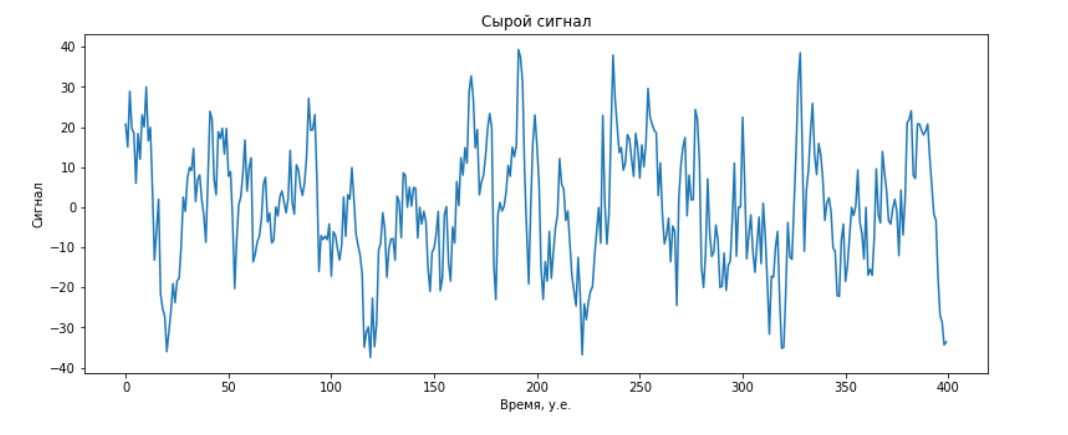
\includegraphics[scale=0.5]{images/8.png}
\end{figure}
Рис.0. Визуализация сигнала ECoG по одному из каналов.
\subsection{Анализ модели}
Сгенерировать дополнительные признаки экспоненциированием предыдущих. Опытным путем подобрать оптимальную размерность латеннтного пространства для алгоритма PLS. Обучить модели PLS, AR, SARIMAX, LR. Перебрать по сетке параметр альфа для блендинга. Сравнить результаты.
\subsection{Выполнение}
После генерации признаков и применения алгоритма PLS получены на тренировочных данных следующие предсказания:

\begin{figure}[H]
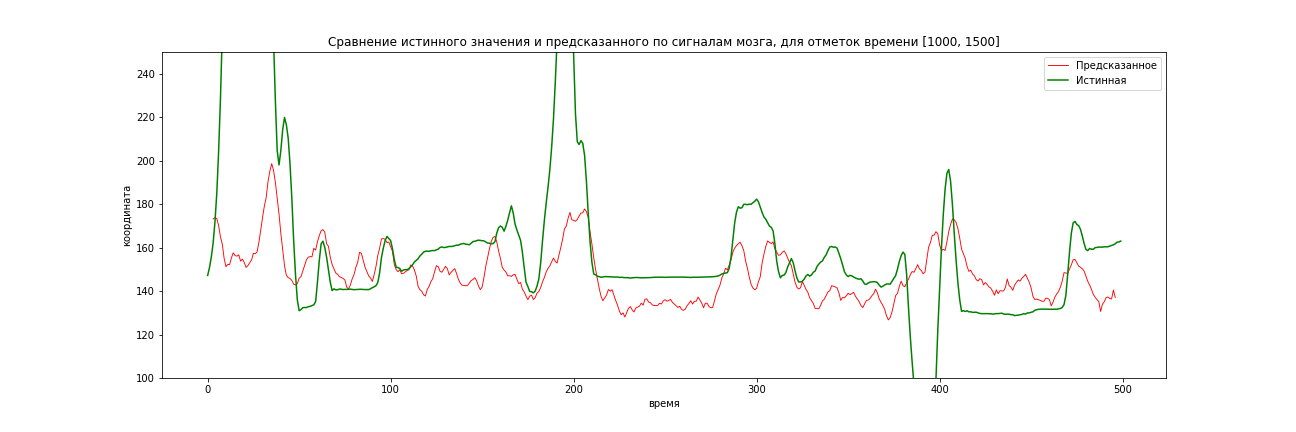
\includegraphics[scale=0.34]{images/1.png}
\end{figure}
Рис.1. Предсказание координаты моделью PLS по временным рядам ативности мозга $\mathbf{X}$
\begin{figure}[H]
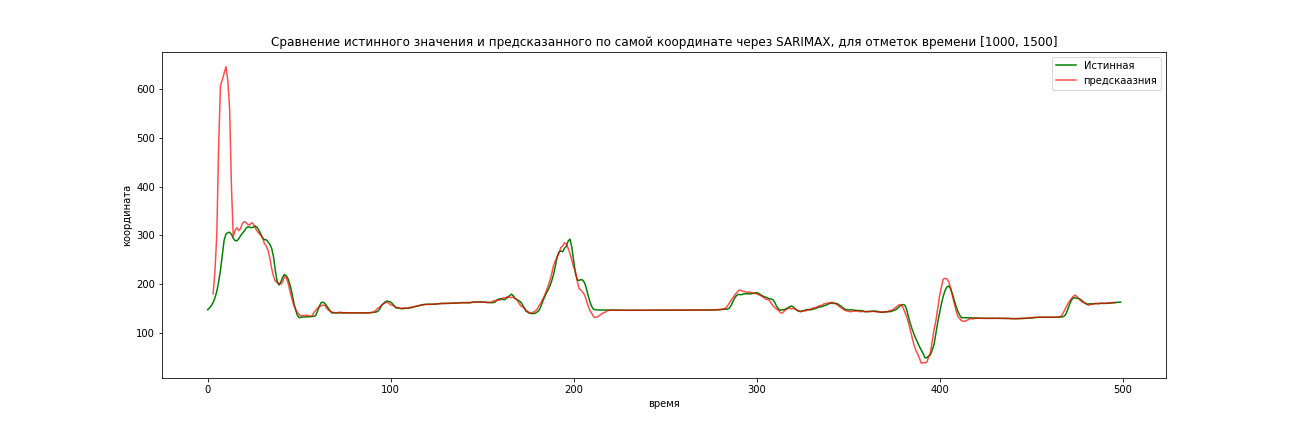
\includegraphics[scale=0.34]{images/2.png}
\end{figure}
Рис.2. Предсказание координаты моделью SARIMAX.
\begin{figure}[H]
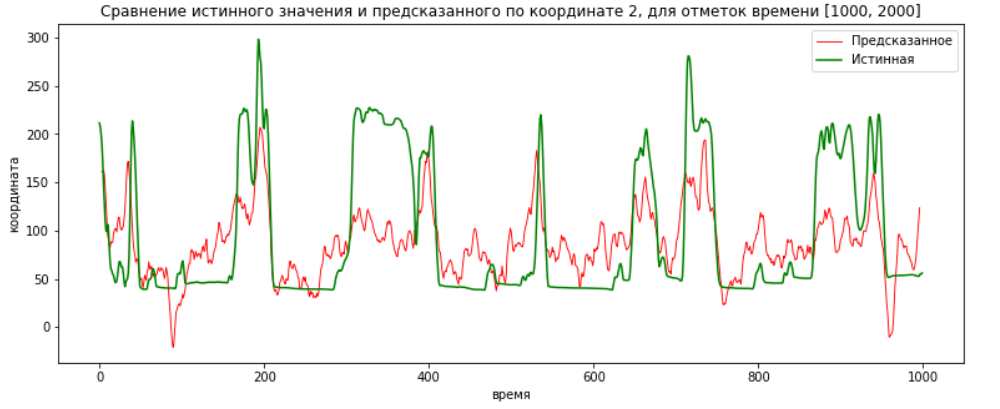
\includegraphics[scale=0.34]{images/3.png}
\end{figure}
Рис.3. Результат блендинга моделей, $\alpha = 0.86$.
\begin{figure}[H]
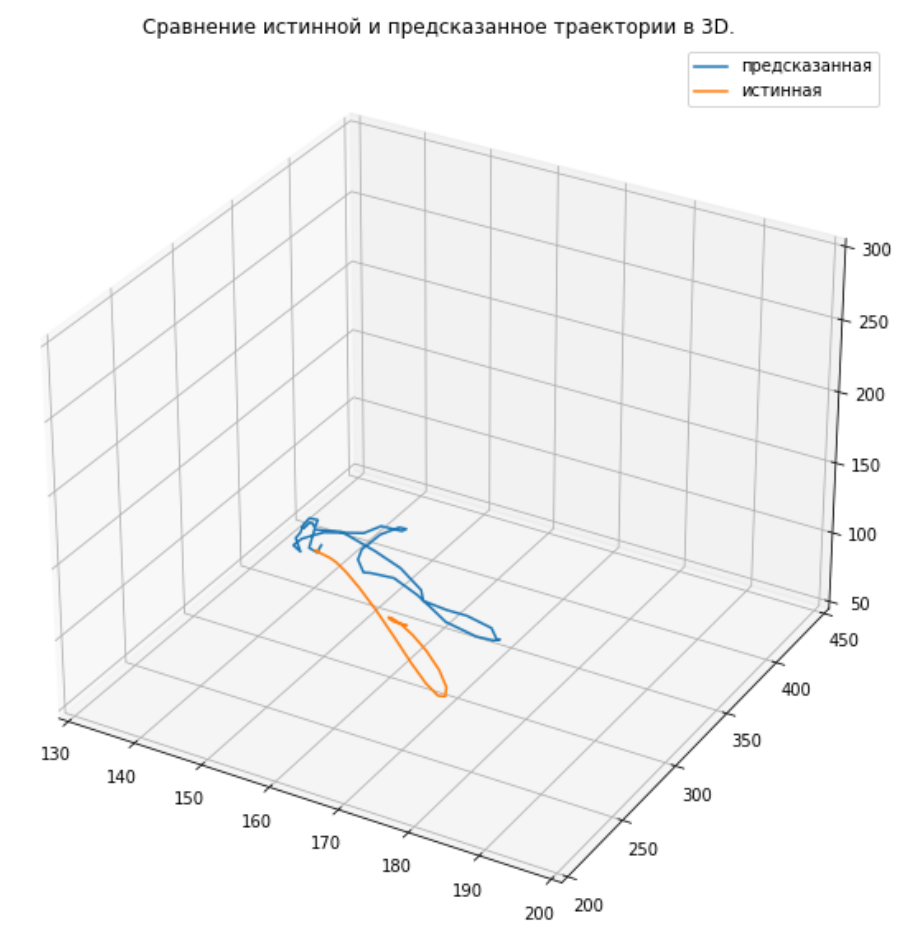
\includegraphics[scale=0.34]{images/4.png}
\end{figure}
Рис.4. Предсказание координаты моделью AR.
\begin{figure}[H]
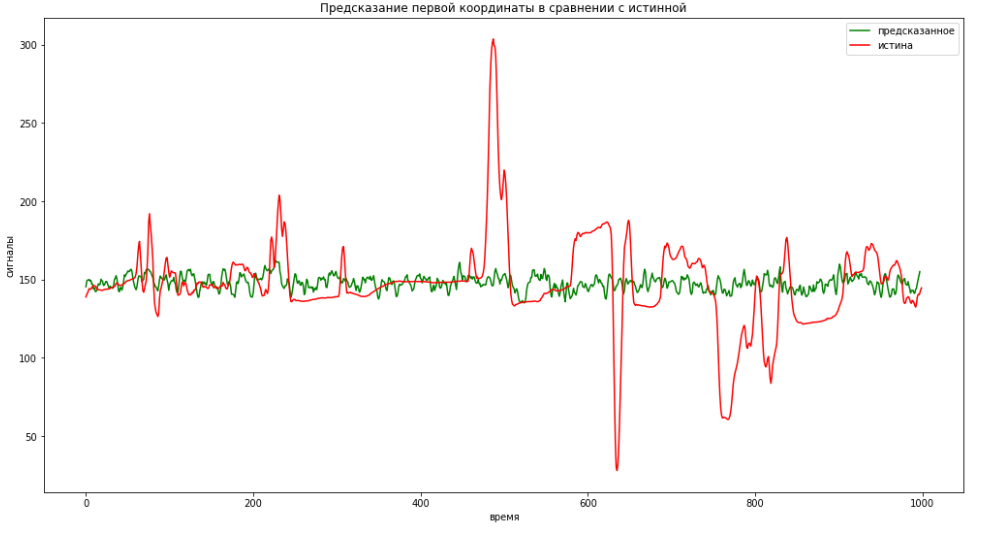
\includegraphics[scale=0.34]{images/5.png}
\end{figure}
Рис.5. Анализ ошибки в зависимости от коэффициента $\alpha$ моделей SARIMAX и PLS.
\begin{figure}[H]
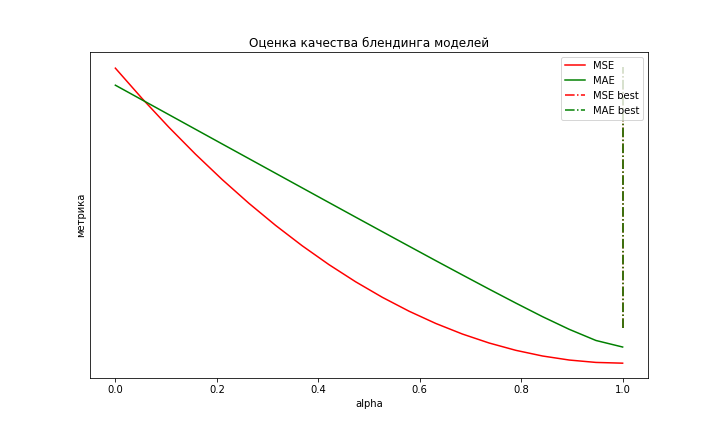
\includegraphics[scale=0.34]{images/6.png}
\end{figure}
Рис.6. Анализ ошибки в зависимости от коэффициента $\alpha$ моделей AR и PLS.



\section{Анализ ошибок}
Рассматривается прогнозирование временного ряда координаты кисти, по прошлым точкам траектрии. Предлагается сравнить пять модели --- $PLS$ в чистом виде, $SARIMAX$ в чистом виде и их микс. А так же $AR$ в чистом виде и его блендинг с $PLS$. Сравнение происходит по метрикам $MSE, MAE$.
\begin{figure}[H]
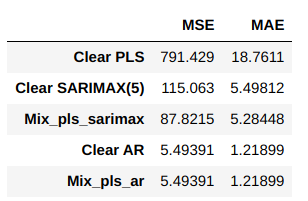
\includegraphics[scale=1]{images/7.png}
\end{figure}
Как видно, микс моделей SARIMAX и PLS дает лучший результат, чем каждая из них поотдельности. Но модель AR сама по себе настолько хороша, что даже блендинг с PLS не улучшает предсказание, а только портит. Можно сделать вывод, что простая AR лучшая модель.
\section{Заключение}
В ходе работы былы предложены и экспериментально проверены разные модели, а так же согласование моделей. Исходя из ошибкок предсказаний утверждается, что предсказание обычной авторегрессией дает гораздо меньшую ошибку чем другие модели и их объединения. Таким образом следует рассматривать вариацию задачи, когда при тестировании моделей тестовый ряд координат прошлых значений не доступен, а доступен только ряд при обучении. 


\nocite{*}
\bibliographystyle{plain}
\bibliography{references}



\end{document}
